\section{Konzept}
%TODO Beschreiben dass Pflanzen in Kreis stehen müssen.
    \subsection{Architektur}
    WateringOfThings besteht aus aus vier Haupt-Komponenten: 
   \begin{itemize}
       \item Microcontroller
           \begin{itemize}
               \item Bewässern der Pflanzen
               \item Erheben der Feuchtigkeitswerte der Blumenerde
           \end{itemize}
       \item MQTT-Broker
           \begin{itemize}
               \item Bidirektionale, leichtgewichtige Kommunikation zwischen Server und Microcontroller
               \item Informiert Server über Daten der Microcontroller
               \item Informiert ausgewählten Microcontroller über Befehle vom Server
           \end{itemize}
       \item REST API
           \begin{itemize}
               \item Informiert Microcontroller in regelmäßigen Abständen die Feuchtigkeitswerte zu nehmen
               \item Speicherung aller Daten (Pflanzen, Feuchtigkeitswerte) in SQLite-Datenbank
               \item Bereitstellung aller Daten im JSON-Format via REST API
           \end{itemize}
    \item App
        \begin{itemize}
            \item Eingabeschnittstelle für Nutzer
            \item Visualisierung der Informationen
        \end{itemize}
   \end{itemize}
    \begin{figure}[H]
        \centering
        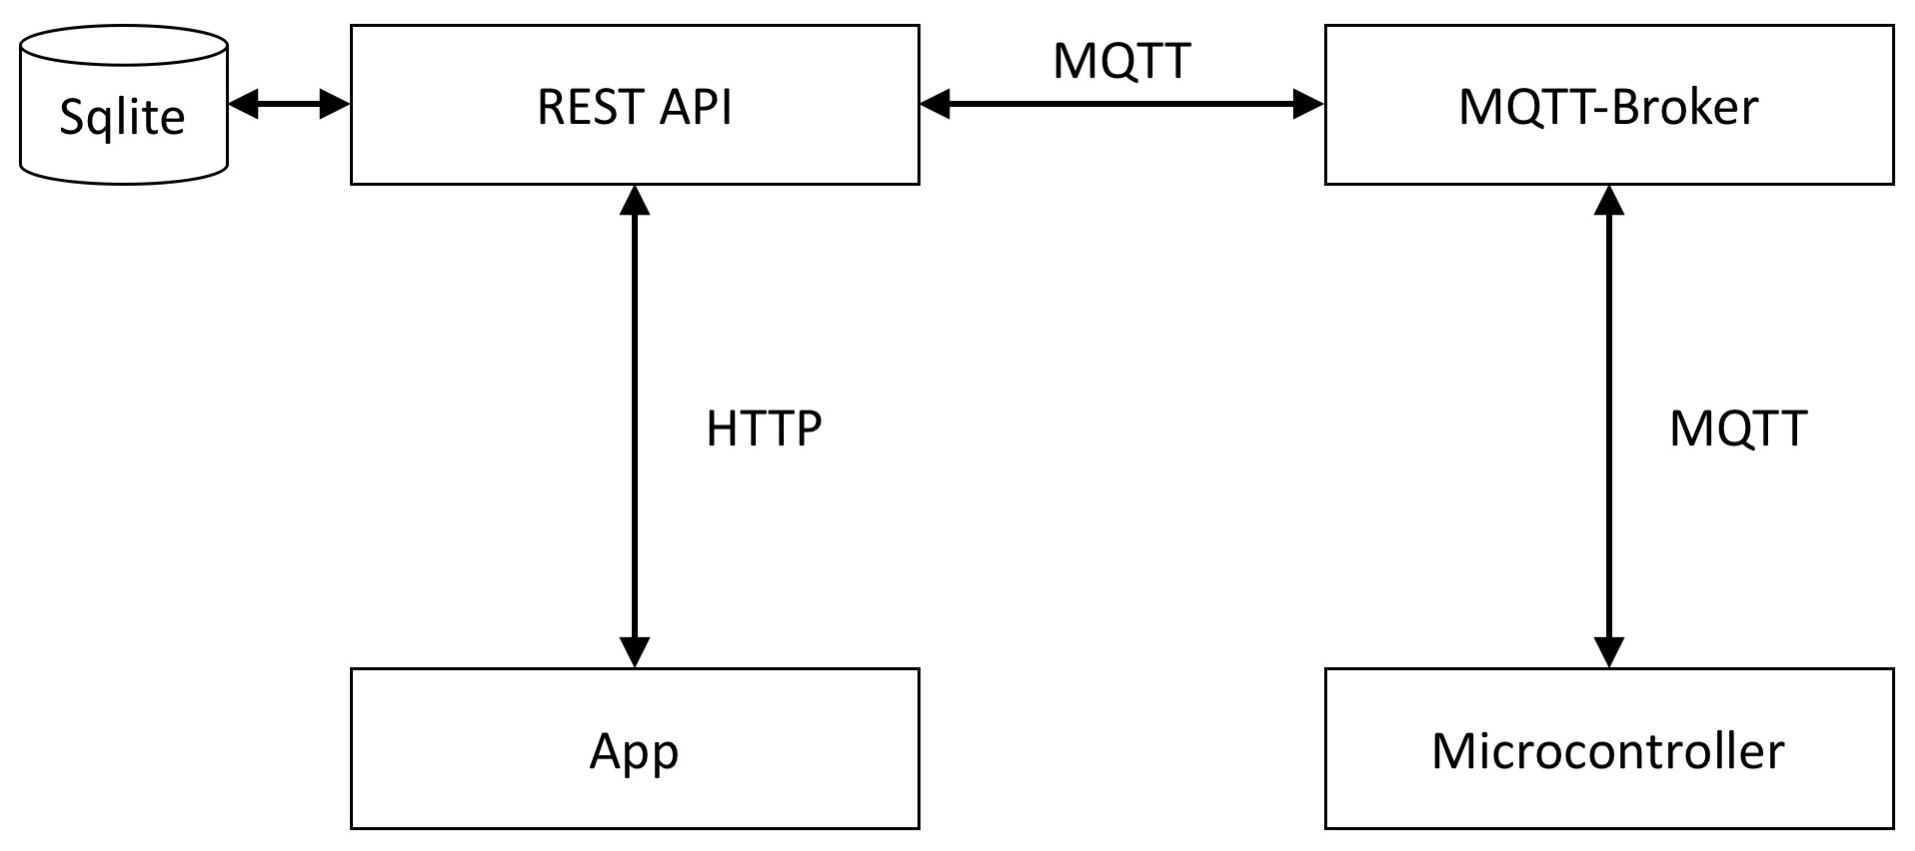
\includegraphics[width=0.7\linewidth]{../Pictures/Konzept/Architecture}
        \caption{Projektarchitektur}
        \label{fig:architecture}
    \end{figure}
    
    \subsection{Datenmodell}
    
     \begin{minipage}{\textwidth}
        Microcontroller\\
        \begin{tabularx}{\linewidth}{|l|l|X|}
            \hline
            Attribut & Datentyp & Beschreibung\\
            \hline
            id & String & Eindeutiger, sicherer Token zur Authentifizierung des Microcontrollers \\
            \hline                              
        \end{tabularx}
    \end{minipage}

\vspace{0.5cm}

     \begin{minipage}{\textwidth}
        Plant\\
          \begin{tabularx}{\linewidth}{|l|l|X|}
              \hline
            Attribut & Datentyp & Beschreibung\\
            \hline
            id & Int & Eindeutige ID der Pflanze \\
            name & String & Frei wählbarer Name für die Pflanze \\
            pin & Int & \begin{tabular}[t]{@{}ll}
            Pin am Microcontroller über den der \\Feuchtigkeitssensor mit der Pflanze verbunden ist \\
            \end{tabular}\\
            position & Int & Position der Pflanze in der Aufstellung in Grad \\
            moistureTreshold & Float & Wert unter dem die Pflanze als trocken gilt \\
            latestMoistureValue & Float & Letzter gemessener Trockenheitswert der Pflanze  \\
            \hline                              
        \end{tabularx}
    \end{minipage}

\vspace{0.5cm}

     \begin{minipage}{\textwidth}
        MoistureValue\\
        \begin{tabularx}{\linewidth}{|l|l|X|}
            \hline
            Attribut & Datentyp & Beschreibung\\
            \hline
            date & Long & Timestamp, wann der Wert erhoben wurde \\
            value & Float & Erhobener Feuchtigkeitswert \\
            \hline                              
        \end{tabularx}
    \end{minipage}
    
    \subsection{Mobile Applikation}

        \subsubsection{React Native}
Ziel dieser Applikation ist es Nutzern eine einfache Möglichkeit zu geben ihre Pflanzen auch im Urlaub versorgen zu können. Um möglichst viele Nutzer mit dieser App zu erreichen wurde eine Entwicklung für die Android als auch für die iOS Plattform angestrebt. Um nicht für beide Plattformen eine eigene App entwickeln zu müssen und damit den doppelten Aufwand für die Entwicklung zu haben, wurde eine Cross-Plattform angestrebt. Die Technologie, welche dies mit nativen Komponenten am besten vereint ist React Native. Des machte eine schnelle Entwicklung für beide Plattformen möglich. 
        
        \subsubsection{Views}\label{views}
Die WateringOfThings App besteht aus fünf verschiedenen Ansichten, Views. Diese führen den Nutzer durch die Anwendung für die oben beschriebenen Use Cases. \\

Beim ersten Start der App wird der Nutzer nach der Eingabe einer Microcontroller-Id gefragt, wie in View \ref{microcontroller} zu sehen. Diese kann von der Hardwarekomponente abgelesen werden. Die Microcontroller-Id wird daraufhin von der App gespeichert. Der Nutzer kann die Id jeder Zeit unter dem Punkt \textit{Settings} ändern. Der erste View und der Settingsview sind dabei gleich. Zu jedem Microcontroller kann der Nutzer anschließend Pflanzen hinzufügen.  
\begin{figure}[H]
    \centering
    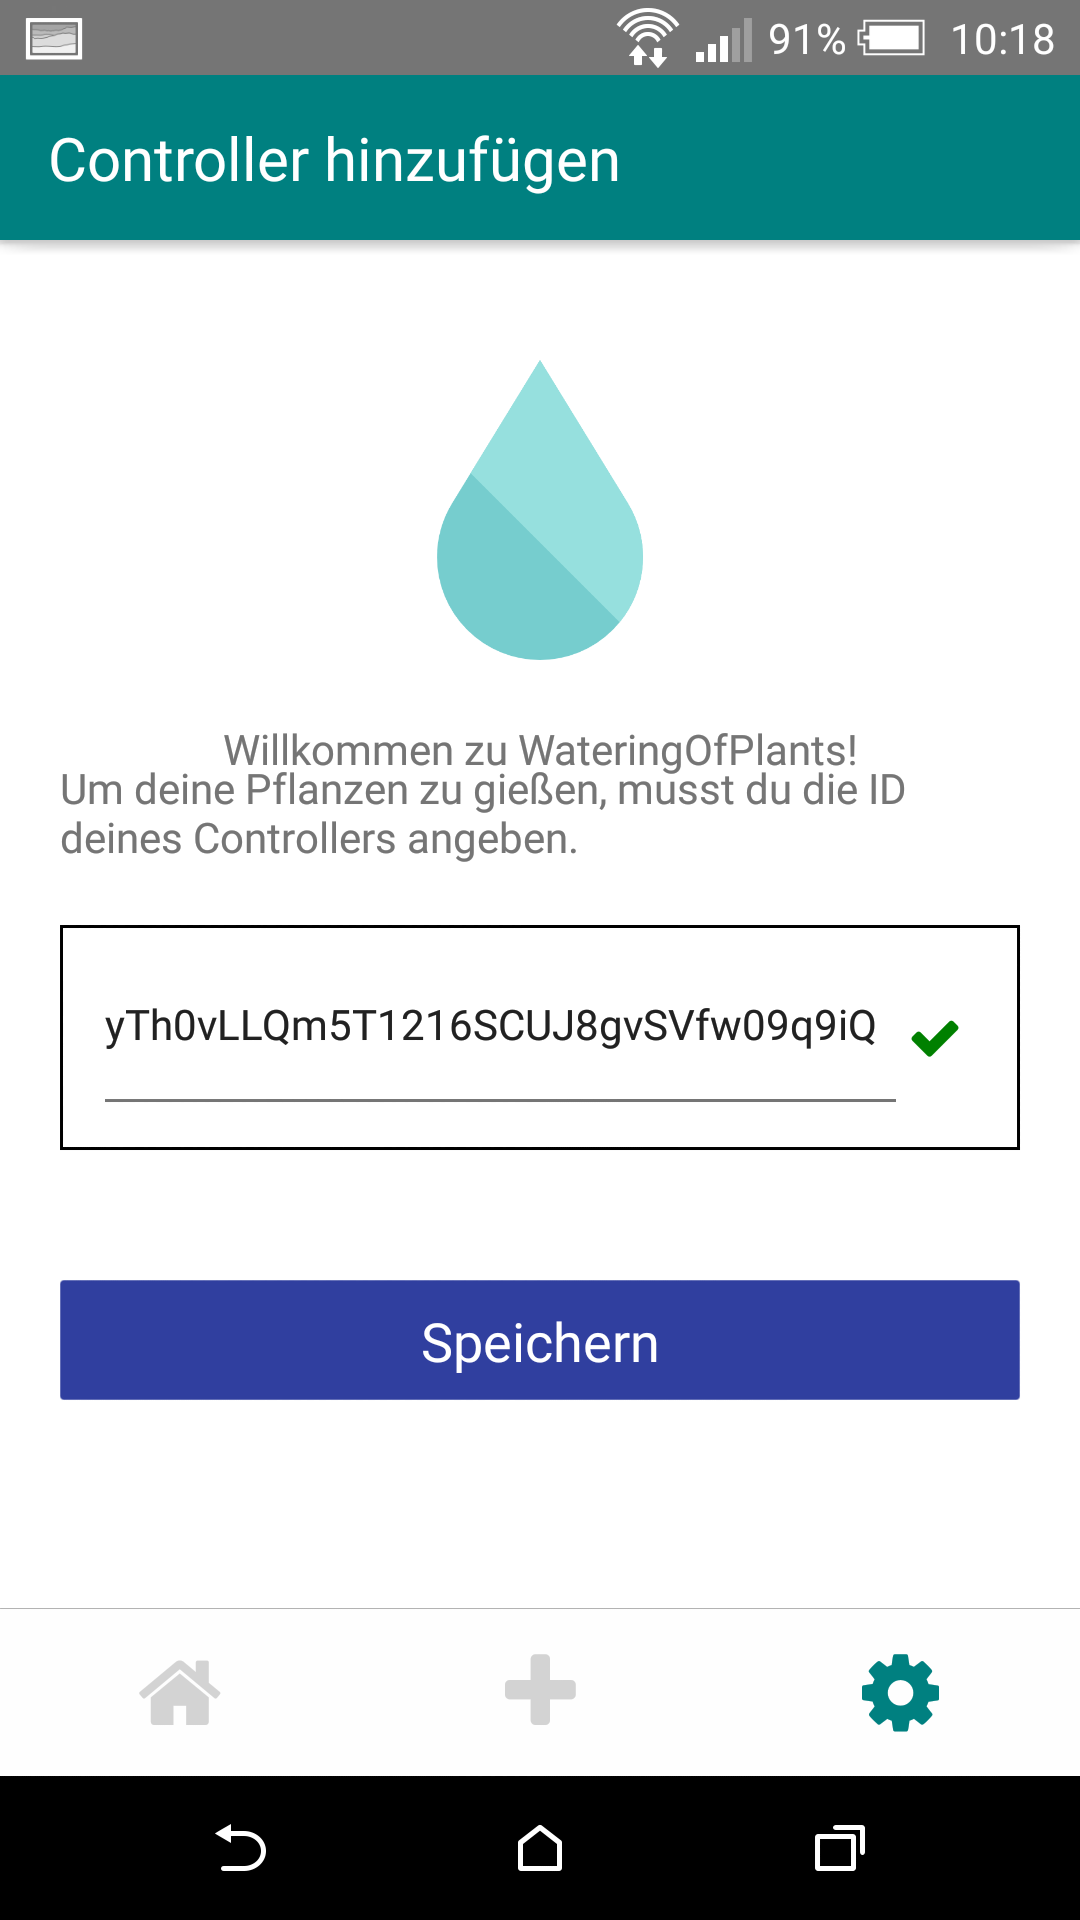
\includegraphics[scale=0.4]{Views/microcontroller.png}
    \caption{Microcontroller-Id hinzufügen}
    \label{microcontroller}
\end{figure}

Der Nutzer hat die Möglichkeit zu einer Microcontroller-Id Pflanzen hinzuzufügen, wie in View \ref{add}. Hierzu kann der Nutzer ein eigenes Bild der Pflanze aus seiner Galerie auswählen. Wird kein Bild ausgewählt wird ein Standardbild angezeigt. Für die Pflanze kann ein Name vergeben werden, z.B. Basilikum. Der Pin ist der Anschluss am Microcontroller. Über ihn kann der Feuchtigkeitssensor mit der Pflanze verbunden werden. Da die Pflanzen im Kreis um den Microcontroller aufgestellt werden, muss die Position angegeben werden. Diese wird in der App in Grad eingegeben. Weitere Information sind im Datenmodell zu finden. \\

Des Weiteren kann ein Trockenheitsschwellwert für die Pflanze angegeben werden. Jede Pflanze braucht unterschiedlich viel Wasser. Um bestimmen zu können wann eine Pflanze das nächste mal gegossen werden sollte, ist der Schwellwert einstellbar. Braucht eine Pflanze wenig Wasser, wie zum Beispiel ein Kaktus, wird der Slider etwas weiter nach links bewegt. Braucht die Pflanze mehr Wasser, wird der Slider nach rechts bewegt. \\

Über eine Validierung wird sichergestellt, dass der Nutzer nur valide Eingaben machen kann. Ist die Eingabe nicht möglich wird ein rotes Ausrufezeichen angezeigt. Ist die Eingabe valide wird ein grüner Haken angezeigt. Erst wenn alle Eingaben valide sind kann die Pflanze gespeichert werden. 

\begin{figure}[H]
    \centering
    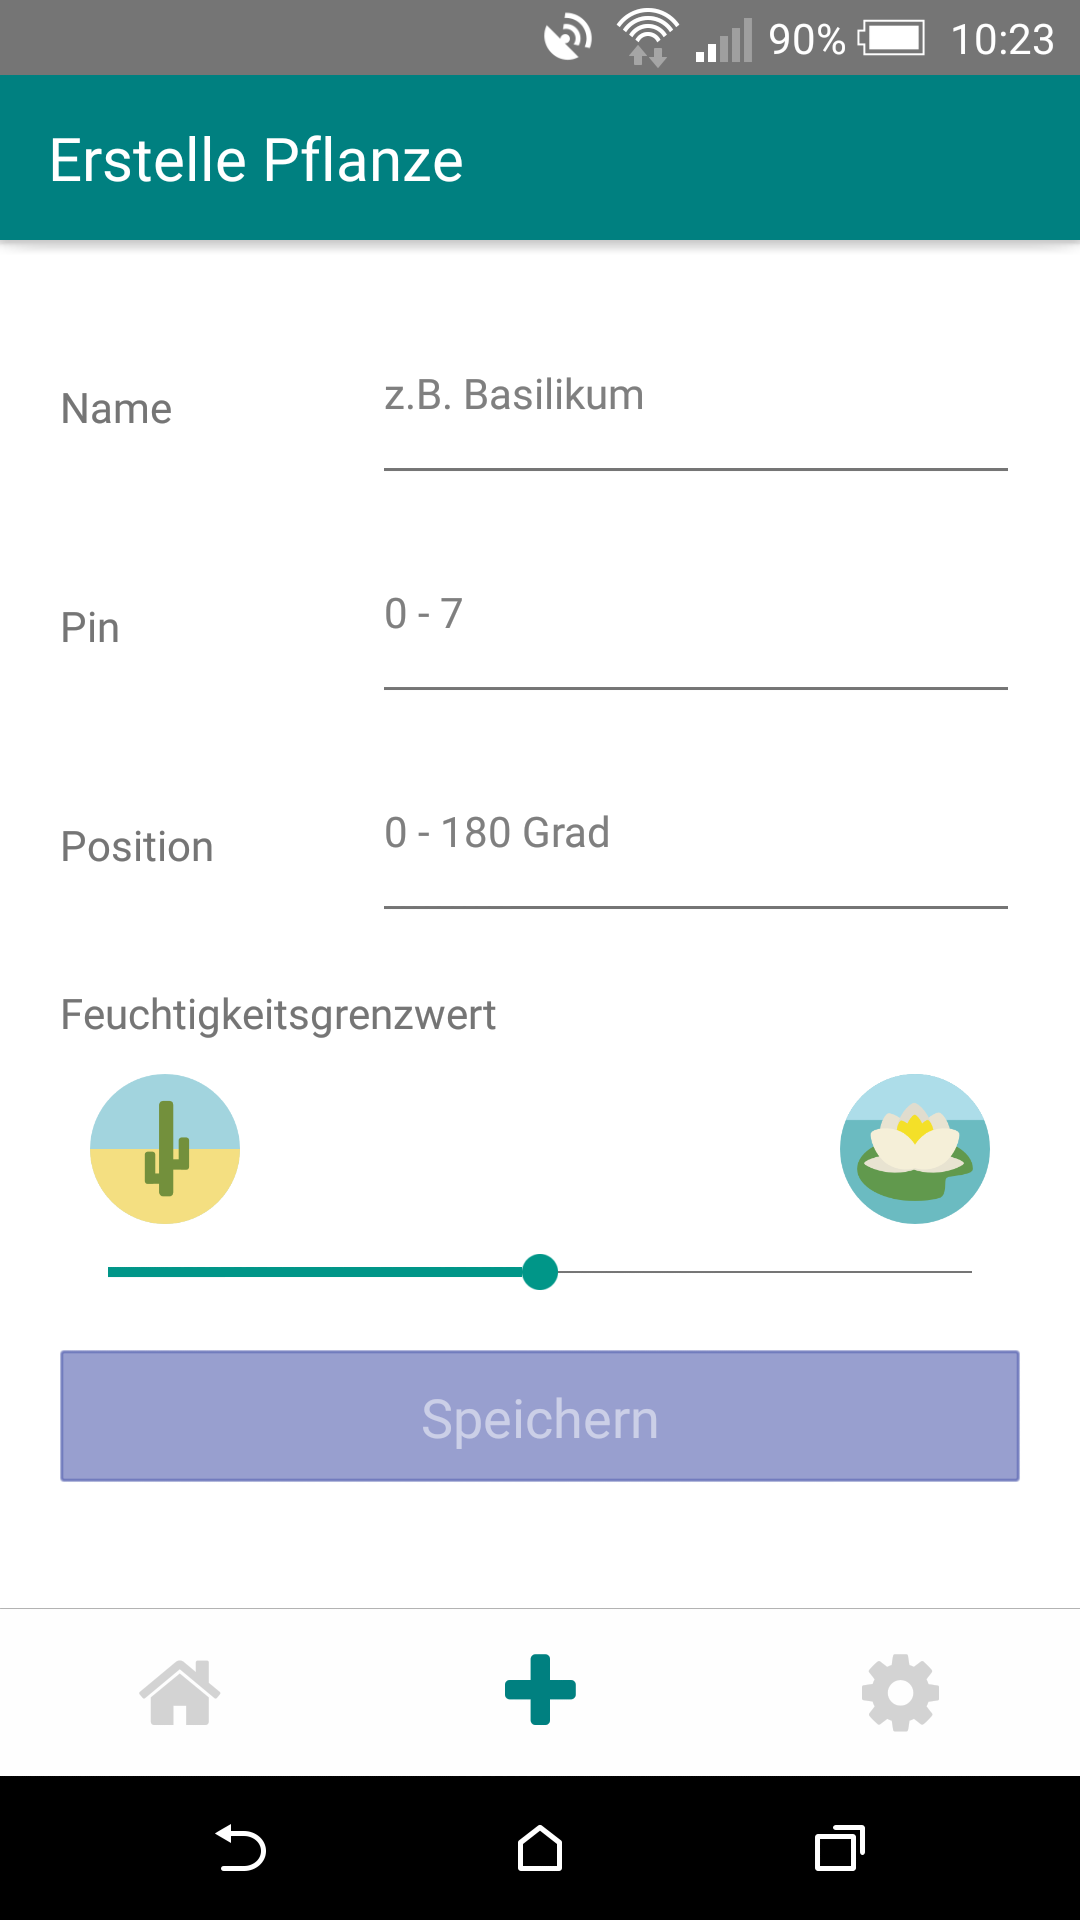
\includegraphics[scale=0.4]{Views/add.png}
    \caption{Pflanze hinzufügen}
    \label{add}
\end{figure}

Alle Pflanzen werden in einer Liste dargestellt, dies ist in View \ref{list} dargestellt. Die Pflanzen werden vom Nutzer zu einer bestimmten Microcontroller-Id hinzugefügt. Der View teilt sich in zwei Listen, eine für zu trockene Pflanzen und eine für gesunde Pflanzen. Fällt der gemessene Trockenheitswert der Pflanze unter ihren Schwellwert, wird die Pflanze in der Liste für Pflanzen angezeigt, die zu trocken sind. Dem Nutzer ist mithilfe der Listen schnell ersichtlich welche Pflanzen gegossen werden sollten und kann selbst entscheiden wann der beste Zeitpunkt ist. Die Pflanzen werden mit ihrem gespeicherten Bild angezeigt, ist kein Bild gespeichert wird ein Standardbild angezeigt. In der oberen Navigationsleiste wird der Name der App mit Logo dargestellt. Zusätzlich hat man in der Navigation die Möglichkeit eine Pflanze hinzuzufügen. Die untere Tableiste ist in allen Views, außer dem Startview gleich. Der Nutzer kann mit \textit{Home} stets zu der Listenansicht zurück navigieren. Mit dem Tab \textit{Add} kann der Nutzer eine neue Pflanze anlegen und im \textit{Settings} Tab die Microcontroller-Id ändern.
\begin{figure}[H]
    \centering
    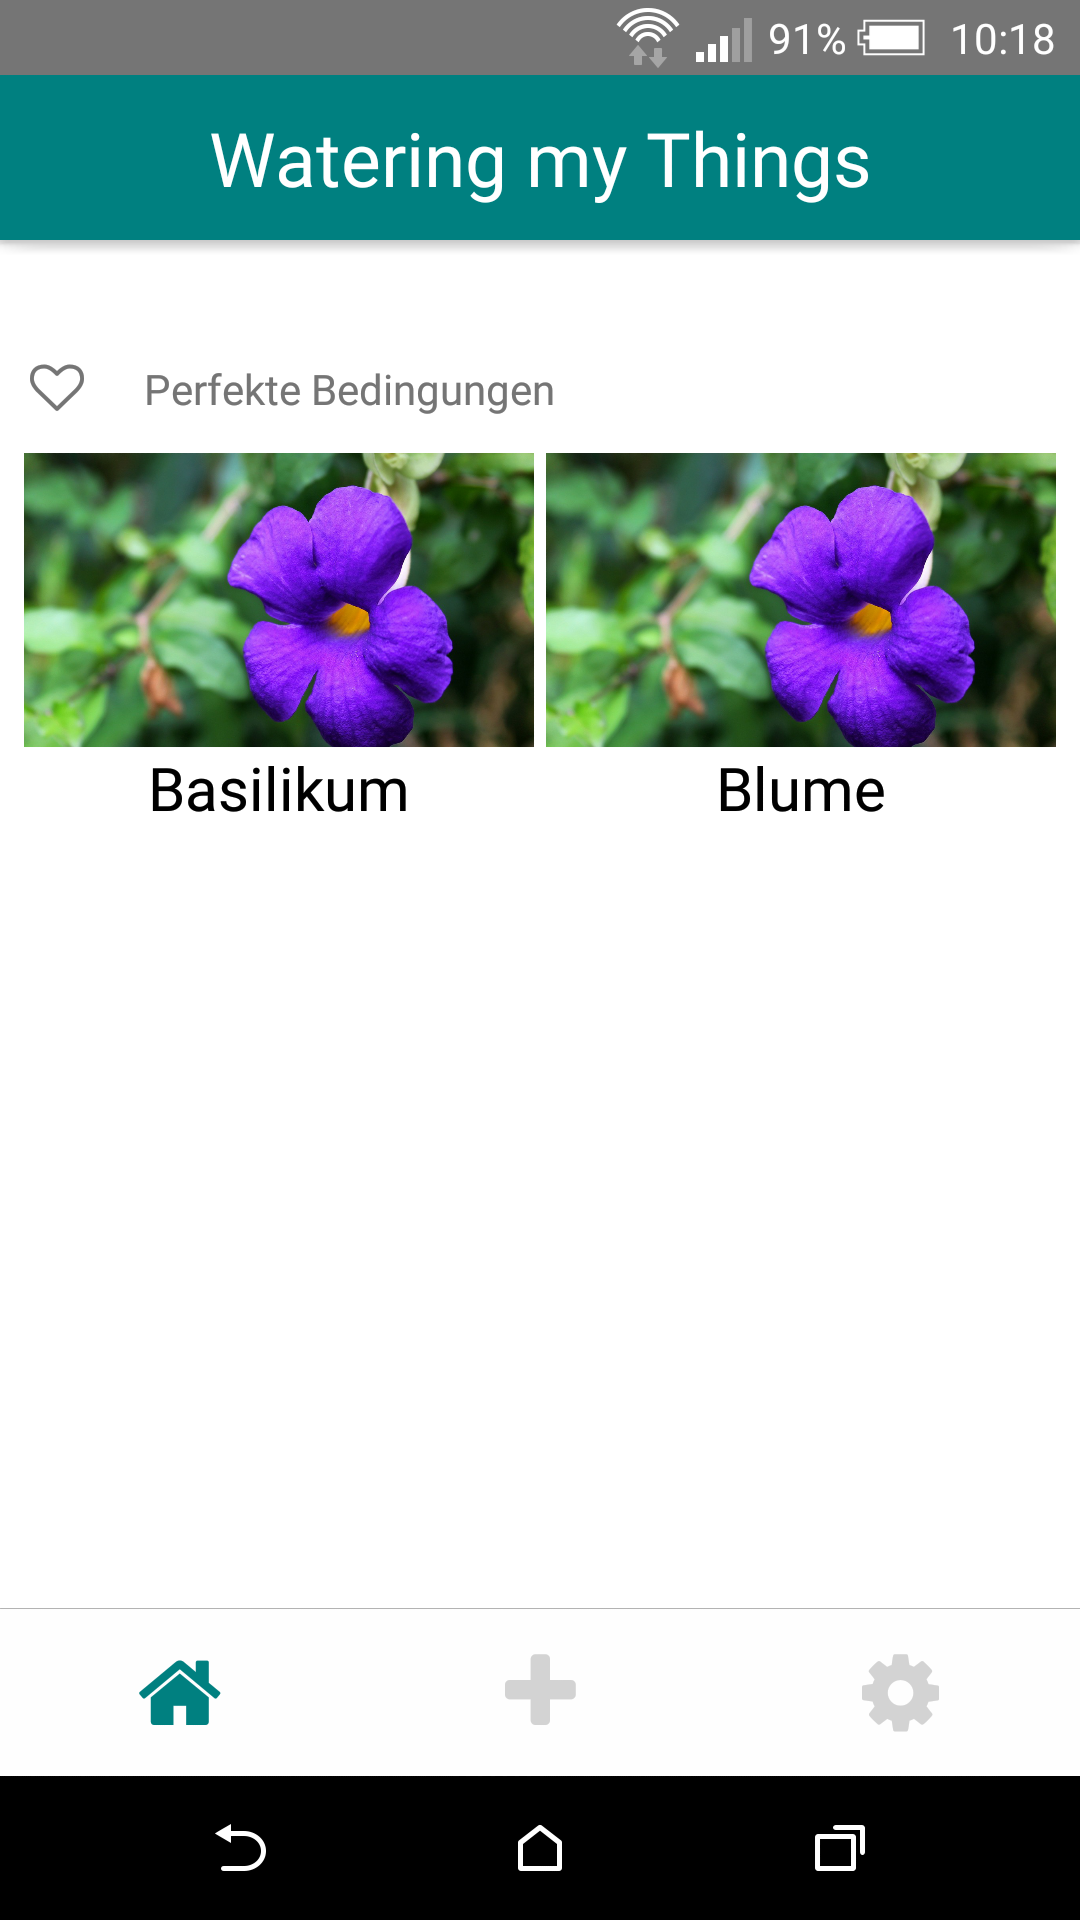
\includegraphics[scale=0.4]{Views/list.png}
    \caption{Liste der Pflanzen}
    \label{list}
\end{figure}

Der Nutzer hat die Möglichkeit seine Pflanzen aus der Liste anzuklicken, damit kommt er auf die Detailseite, wie in View \ref{plant}. In der Detailseite für die einzelnen Pflanzen wird der Trockenheitsstatus der Pflanze genauer angezeigt. Der Name der Pflanze wird oben in Navigation angezeigt. Rechts davon hat der Nutzer mit dem Änderungs-Icon die Möglichkeit die Daten der Pflanze zu bearbeiten. Der Bearbeitungs-View ist ähnlich dem Hinzufügen-View, nur mit schon ausgefüllten Feldern. \\

Über den \textit{Water-Button} hat der Nutzer die Möglichkeit die Pflanze zu gießen. Hierfür wird er auf den nächsten View weitergeleitet. 

\begin{figure}[H]
    \centering
    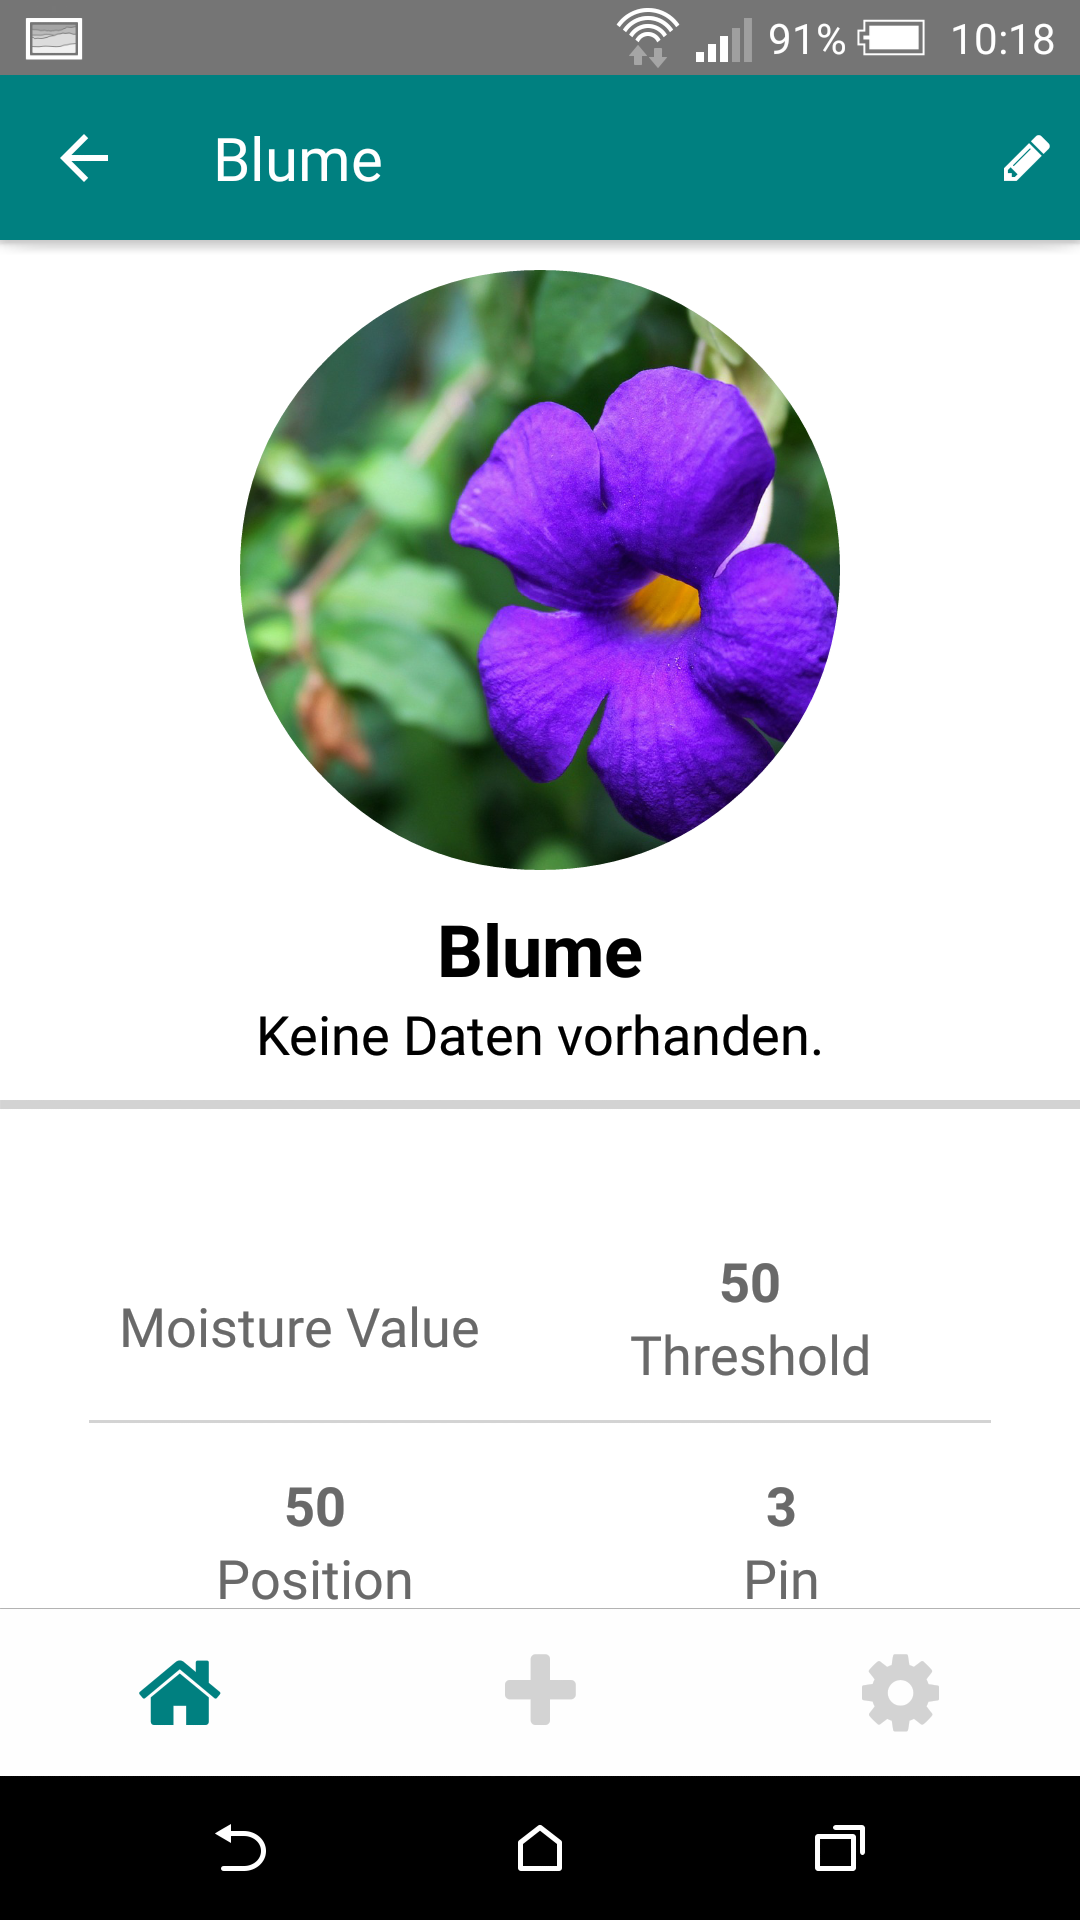
\includegraphics[scale=0.4]{Views/plant.png}
    \caption{Pflanzen-Detail Seite}
    \label{plant}
\end{figure}

Im View zum gießen der Pflanzen, wie in View \ref{water} zu sehen, sieht man noch einmal den Trockenheitsstatus der Pflanze. Darunter hat man die Möglichkeit eine bestimmte Menge an Wasser auszuwählen mit der die Pflanze gegossen werden soll. 
\begin{figure}[H]
    \centering
    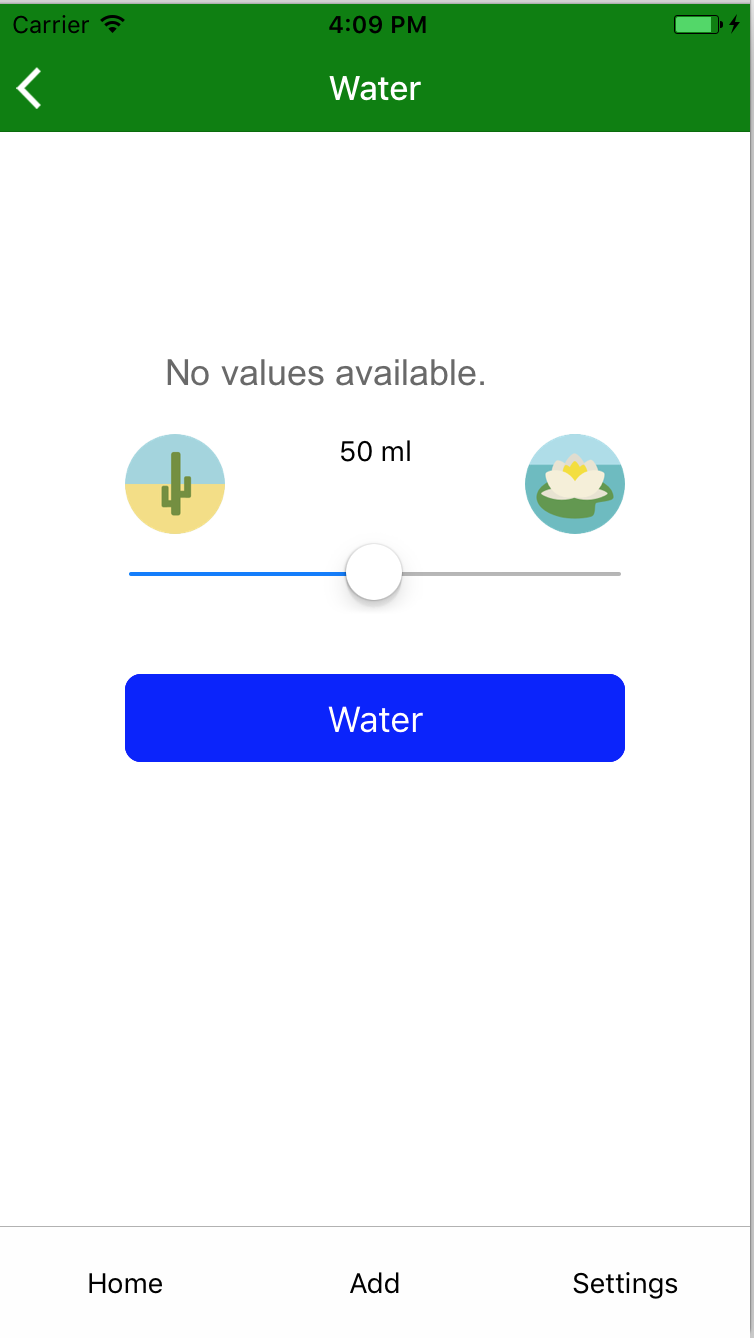
\includegraphics[scale=0.4]{Views/water.png}
    \caption{Pflanze gießen}
    \label{water}
\end{figure}

    \subsection{REST-API}

        \subsubsection{Django}
        \subsubsection{Ressourcen}
        \newcommand{\tabitem}{~~\llap{\textbullet}~~}
     \begin{minipage}{\textwidth}
             GET controller/\{controllerID\}/ 
        
          \begin{tabularx}{\textwidth}{lX}
                \toprule Beschreibung & Überprüft Validität der Controller-ID \\
                URL-Parameter & controllerID: zu überprüfende ID des Controllers \\
                Body & - \\
                Response & \{ "exists": true/false\}
            \end{tabularx}
    \end{minipage}\\\\
        
     \begin{minipage}{\textwidth}
            GET controller/\{controllerID\}/plant/ 

          \begin{tabularx}{\textwidth}{lX}
                \toprule Beschreibung & Alle Pflanzen des Microcontrollers \\
                URL-Parameter & controllerID: ID des Controllers mit dem die Pflanzen verbunden sind \\
                Body & - \\
                Response & Liste von Pflanzen
            \end{tabularx}
    \end{minipage}\\\\
        
     \begin{minipage}{\textwidth}
             POST  controller/\{controllerID\}/plant/ 
         
          \begin{tabularx}{\textwidth}{lX}
             \toprule Beschreibung & Erstellt eine neue Pflanze \\
             URL-Parameter & controllerID: ID des Controllers mit dem die Pflanzen verbunden sind \\
             Body & Zu erstellende Pflanze ohne ID \\
             Response & Erstellte Pflanze mit ID
         \end{tabularx}
    \end{minipage}\\\\
     
     \begin{minipage}{\textwidth}
              GET  controller/\{controllerID\}/plant/\{plantID\} 
          
          \begin{tabularx}{\textwidth}{lX}
              \toprule Beschreibung & Alle Informationen zu einer spezifischen Pflanze \\
              URL-Parameter & 
                  \begin{tabular}[t]{ll}
                       \tabitem controllerID: ID des Controllers mit dem die Pflanzen verbunden sind \\ 
                       \tabitem plantID: Eindeutige ID der angefragten Pflanze
                  \end{tabular}\\
              Body & - \\
              Response & Pflanzenobjekt
          \end{tabularx}
    \end{minipage}\\\\
          
     \begin{minipage}{\textwidth}
              PUT controller/\{controllerID\textgreater/plant/\{plantID\} 
          
            \begin{tabularx}{\textwidth}{lX}
              \toprule Beschreibung & Updated eine existierende Pflanze \\
              URL-Parameter & 
              \begin{tabular}[t]{ll}
                  \tabitem controllerID: ID des Controllers mit dem die Pflanzen verbunden sind \\ 
                  \tabitem plantID: Eindeutige ID der zu updatenden Pflanze
              \end{tabular}\\
              Body & Geändertes Pflanzenobjekt \\
              Response & Geändertes Pflanzenobjekt
          \end{tabularx}
    \end{minipage}\\\\
      
     \begin{minipage}{\textwidth}
         
              DELETE controller/\{controllerID\}/plant/\{plantID\}/ 
          
          \begin{tabularx}{\textwidth}{lX}
              \toprule Beschreibung & Löschen einer Pflanze \\
              URL-Parameter & 
              \begin{tabular}[t]{ll}
                  \tabitem controllerID: ID des Controllers mit dem die Pflanzen verbunden sind \\ 
                  \tabitem plantID: Eindeutige ID der zu löschenden Pflanze
              \end{tabular}\\
              Body & - \\
              Response & -
          \end{tabularx}
        \end{minipage}\\\\
      
     \begin{minipage}{\textwidth}
         
              GET  controller/\{controllerID\}/plant/\{plantID\}/moisture 
          
          \begin{tabularx}{\textwidth}{lX}
              \toprule Beschreibung & Abfragen aller Feuchtigkeitsmessungen für eine Pflanze \\
              URL-Parameter & 
              \begin{tabular}[t]{ll}
                  \tabitem controllerID: ID des Controllers mit dem die Pflanzen verbunden sind \\ 
                  \tabitem plantID: Eindeutige ID der Pflanze
              \end{tabular}\\
              Body & - \\
              Response & Liste an Feuchtigkeitswerten
          \end{tabularx}
        \end{minipage}\\
      
     \begin{minipage}{\textwidth}
             
      POST controller/\{controllerID\}/plant/\{plantID\}/water/\{amount\} 
      
          \begin{tabularx}{\textwidth}{lX}
          \toprule Beschreibung & Bewässerung einer Pflanze \\
          URL-Parameter & 
          \begin{tabular}[t]{ll}
              \tabitem controllerID: ID des Controllers mit dem die Pflanzen verbunden sind \\ 
              \tabitem plantID: Eindeutige ID der zu bewässernden Pflanze \\
              \tabitem amount: Wassermenge in Millilitern
          \end{tabular}\\
          Body & - \\
          Response & -
      \end{tabularx}
  \end{minipage}\\

    \subsection{Microcontroller}


        \subsubsection{Kommunikation}
        Zur Kommunikation wird das Protokoll \textit{MQTT} verwendet. MQTT ist ein leichtgewichtiges Nachrichtenprotokoll, welches auf TCP/ IP aufbaut. Es ist wurde speziell für Anwendungen mit geringen Ressourcen sowie für limitierten Bandbreite entworfen. Damit eignet es sich sehr gut für Internet-of-Things-Anwendungen, wird aber auch zunehmend bei mobilen Applikationen genutzt.
        
        MQTT setzt das Publish-Subscribe-Pattern um. Server und Microcontroller sind beide Clients, die sich mit einem gemeinsamen MQTT-Broker verbinden. Dort können sie sich für Benachrichtigungen zu speziellen Themen anmelden (subscribe). Themen werden als URL dargestellt. Inhalte zu einem Thema können veröffentlicht (publish) werden. Der Broker benachrichtigt dann automatisch alle Clients, welche sich für das Thema eingeschrieben haben.
        
        Die Form der gesendeten Daten unterscheidet sich teilweise etwas vom gewohnten Vorgehen mit leistungsstärkeren Geräten. Die Form ist darauf ausgelegt zu jeder Zeit eine minimale Menge an Daten auf dem Microcontroller vorzuhalten sowie diese möglichst leichtgewichtig lesbar zu machen.\\
        
        \begin{minipage}{\textwidth}
            WateringOfPlants/microController/\{controllerID\}/water
            
            \begin{tabularx}{\textwidth}{lX}
                \toprule Beschreibung & Anweisung vom Server eine Pflanze zu bewässern  \\
                URL-Parameter & controllerID: ID des Controllers der die Pflanze bewässern soll\\
                Daten & 
                  \begin{tabular}[t]{ll}
                      \{ \\
                          \tab "position": <position>, \\
                          \tab "time": <time> \\
                      \} \\
                    \tabitem position: Position der Pflanze in Grad \\ 
                    \tabitem time: Zeit in Millisekunden für die die Pumpe aktiviert werden soll
                \end{tabular}\\
            \end{tabularx}
        \end{minipage}\\
    
        WateringOfPlants/microController/\{controllerID\}/measure
        
        \begin{minipage}{\textwidth}
            \begin{tabularx}{\textwidth}{lX}
                \toprule Beschreibung & Anweisung vom Server die Feuchtigkeitswerte zu erheben  \\
                URL-Parameter & controllerID: ID des Controllers der die Werte erheben soll\\
                Daten & 
                \begin{tabular}[t]{ll}
                    \{ \\
                    \tab "pins": [<pinNr>, <pinNr> ... ]>, \\
                    \tab "nrOfPins": <nrOfPins> \\
                    \} \\
                    \tabitem pins: Pins an denen die Feuchtigkeitssensoren angeschlossen sind \\ 
                    \tabitem nrOfPins: Länge des pins-Arrays
                \end{tabular}\\
            \end{tabularx}
        \end{minipage}\\
    
    
        WateringOfPlants/microController/\{controllerID\}/measuredValues/\{pinNr\}
        
        \begin{minipage}{\textwidth}
            \begin{tabularx}{\textwidth}{lX}
                \toprule Beschreibung & Gemessener Feuchtigkeitswert vom Microcontroller  \\
                URL-Parameter &  
                \begin{tabular}[t]{ll}
                    \tabitem controllerID: ID des Controllers, der den Feuchtigkeitswert erhoben hat.\\ 
                    \tabitem pinNr: Pin zu welchem der Feuchtigkeitswert erhoben wurde
                \end{tabular}\\
                Daten & 
                \begin{tabular}[t]{ll}
                    <moistureValue> \\
                    \tabitem moistureValue: Erhobener Feuchtigkeitswert als Double
                \end{tabular}\\
            \end{tabularx}
        \end{minipage}\\
    
        \subsubsection{Aufbau}
        Die Möglichkeit einer Tröpfchenbewässerung wurde verworfen um die Pflanzen eine größere Unterschiede bei der Pflanzenbewässerung sicherstellen zu können. Um trotzdem möglichst viele Pflanzen versorgen zu können, wird ein kreisförmiger Aufbau der Pflanzen vorausgesetzt, wie in Abbildung \ref{fig:position} gezeigt. Damit können von einer Hardwarekomponente acht Pflanzen versorgt werden. \\
        
        Für den Aufbau werden folgende Komponenten mindestens benötigt:
        \begin{itemize}
            \item 1 WLAN-fähiger Microcontroller, der mittels MQTT kommunizieren kann
            \item 1 Wasserschlauch über den das Wasser von der Quelle zur Pflanze geleitet wird
            \item 1 Servomotor, welcher den Schlauch zur entsprechenden Pflanze bewegt
            \item 1 Pumpe, die das Wasser von der Quelle zur Pflanze befördert
           \item 8 Feuchtigkeitssensoren, die den Feuchtigkeitsgehalt der Blumenerde messen
        \end{itemize}
        \begin{figure}
            \centering
            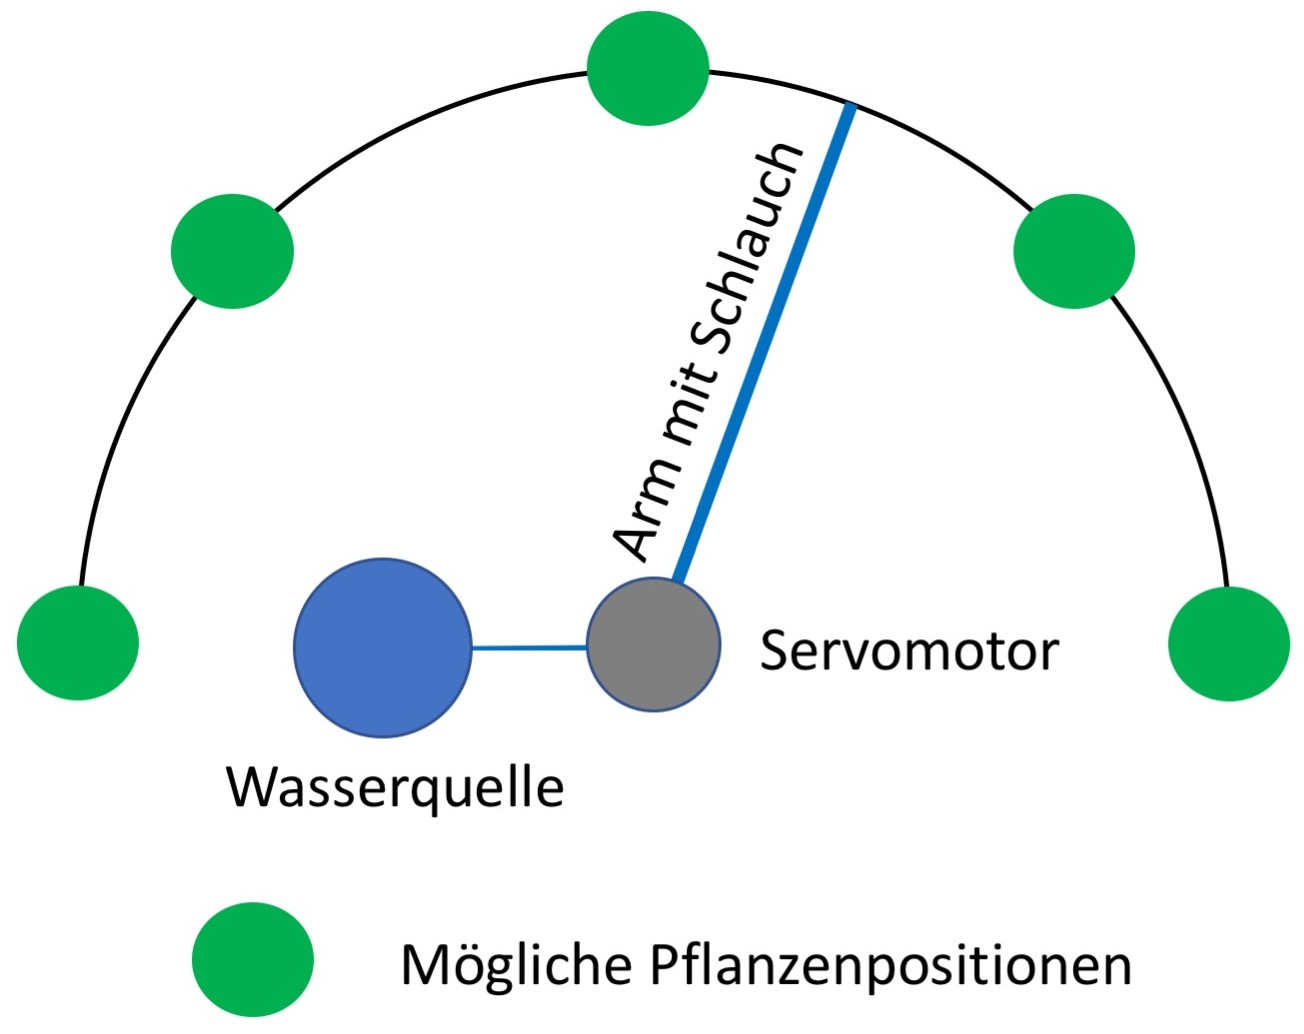
\includegraphics[width=0.6\linewidth]{Pictures/Konzept/Position}
            \caption{Anordnung der Pflanzen}
            \label{fig:position}
        \end{figure}
        
    \subsection{Codequalität}